\chapter{Автоматная модель технологических процессов}

\section{Задача оптимизации технологического процесса}

Пусть имеется следующая информация о реакторе и о его процессе планово-предупредительного ремонта:
\begin{enumerate}
\item Абстрактное описание конструкции реактора и порядка процесса планового-предупредительного ремонта. Данное описание должно быть представлено в виде абстрактного цифрового автомата или композиции таких автоматов. То есть должны быть заданы множество состояний реактора, множество операций, производимых над реактором, функция перехода, указывающая допустимые переходы из одного состояния в другое при приведении операций, а также начальное и конечные состояния реактора  при ремонте. При этом для каждого состояния реактора и каждой операции заданы известные физические характеристики. Назовем такое описание ТА-моделью.
\item Данные для физического моделирования. Данные для физического моделирования представляют собой набор физических характеристик, заданных в ТА-модели, и соответствующие им расчетные характеристики реактора, такие как мощность, температура активной зоны, запас реактивности и т.д. Расчётные характеристики могут быть рассчитаны с помощью эксплуатационных программ либо измерены в ходе предыдущих кампаний. Также для каждого значения должна быть указана физическая допустимость представленных параметров.
\item Функция оптимизации. Данная функция является весовой функцией характеристик операций, производимых над реактором. Она требуется для изменения значимости различных факторов при проведении оптимизации. Поиск оптимального порядка будет производиться по минимальным значениям данной функции.
Обработав исходные данные, метод должен представить на выходе оптимальный согласно функции оптимизации порядок проведения перезагрузки реактора. При этом искомый порядок не должен содержать физически недопустимых состояний реактора.
\end{enumerate}

Рассмотрим порядок работы метода моделирования и оптимизации (см. рис.~\ref{pic:overall}).
\begin{figure}[ht]
  \center{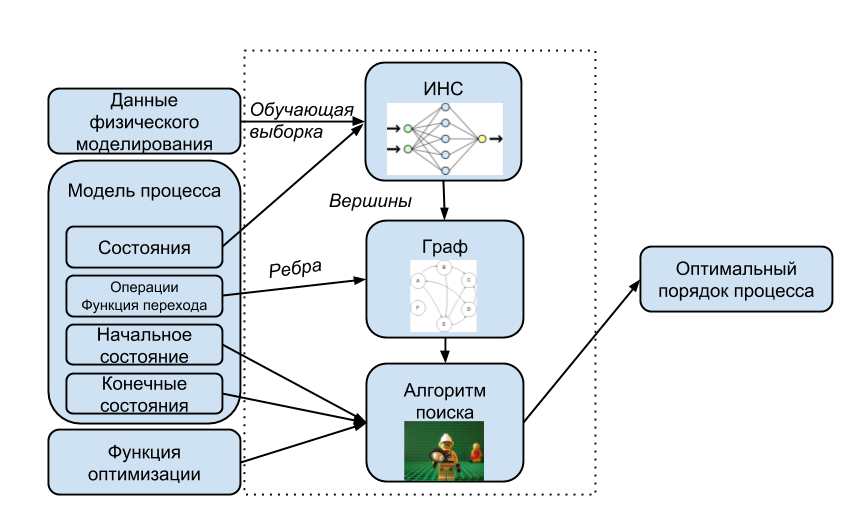
\includegraphics[width=0.8\linewidth]{overall.png}}
  \caption[Обзорная диаграмма процесса моделирования и оптимизации]{Обзорная диаграмма процесса моделирования и оптимизации}
  \label{pic:overall}
  \end{figure}
Искусственная нейронная сеть обучается на данных физического моделирования. После успешного завершения обучения нейронная сеть становится способна аппроксимировать расчётные характеристики реактора на основе физического состояния реактора (состояния ТА-модели реактора), а также принимать решение о физической допустимости состояния.
Множество состояний ТА-модели реактора поэлементно подаются в качестве входного вектора искусственной нейронной сети. Нейронная сеть делит множество состояний на допустимые и недопустимые, дополняя при этом каждое состояние значениями расчетных характеристик. Допустимые состояния составляют узлы графа переходов ТА-модели, остальные отбрасываются.
Между узлами графа переходов устанавливаются направленные ребра, соответствующие множеству операций и функции перехода ТА-модели. По завершению процесса построения имеется граф переходов между допустимыми состояниями реактора.
С помощью алгоритма информированного поиска А* производится поиск кратчайшего пути от начального состояния графа до ближайшего конечного состояния. В качестве информирующей характеристики алгоритма выступает заданная функция активации.
По завершения работы алгоритма поиска имеется множество путей, ведущих кратчайшим путем к каждому из конечных состояний. Путь с минимальным значением функции оптимизации является искомым. \cite{modeling-2014, modeling-2015}



\section{Автоматная модель технологического процесса}

риведем общие понятия и положения теории автоматов, необходимые для построения формальной информационной модели реактора.

\begin{Def}
 Алфавитом $\Sigma$ называют некоторое непустое конечное множество символов.
\end{Def}

\begin{Def}
 Словом называют некоторую конечную (возможно, пустую) последовательность символов алфавита: $\omega = \sigma_1\sigma_2\dots\sigma_l$. 
 Количество символов в слове (число $l$) называют длиной слова. 
 Пустое слово принято обозначать $\varepsilon$.
\end{Def}

\begin{Def}
 Детерминированным конечным автоматом (ДКА) называется пятерка (кортеж) $A = \langle Q, \Sigma, \delta, q_0, F  \rangle$, где:
 \begin{itemize}
  \item [-] $Q$ --- конечное множество состояний;
  \item [-] $\Sigma$ --- алфавит;
  \item [-] $\delta : Q \times \Sigma \rightarrow Q$ --- функция переходов;
  \item [-] $q_0 \in Q$ --- начальное состояние;
  \item [-] $F \subseteq Q$ --- множество терминальных (конечных) состояний.
 \end{itemize}
\end{Def}

Обработка слова $\omega = \sigma_1\sigma_2\dots\sigma_l$ ДКА $A$ происходит следующим образом. 
Сначала автомат $A$ находится в стартовом состоянии $q_0$. 
Затем на каждом шаге обработки автомат считывает очередной символ $sigma_i$ слова $\omega$ и переходит из своего текущего состояния $q$ в состояние $\delta(q; \omega_i)$. 
К моменту, когда все символы входного слова $\omega$ обработаны, автомат находится в некотором состоянии $p$. Говорят, что автомат A принимает слово $\omega$, если $p \in F$, и не принимает в обратном случае.\cite{TA-defs}

Определение ДКА как пятерки объектов с детальным описанием функций переходов слишком сухое и неудобочитаемое.
Существует два более удобных способа описания автоматов.
\begin{enumerate}
 \item \textit{Диаграмма переходов}, которая представляет собой граф.
 \item \textit{Таблица переходов}, дающая табличное представление функции $\delta$.
 Из нее очевидны состояния и входной алфавит.
\end{enumerate}

\begin{figure}[ht]
\center{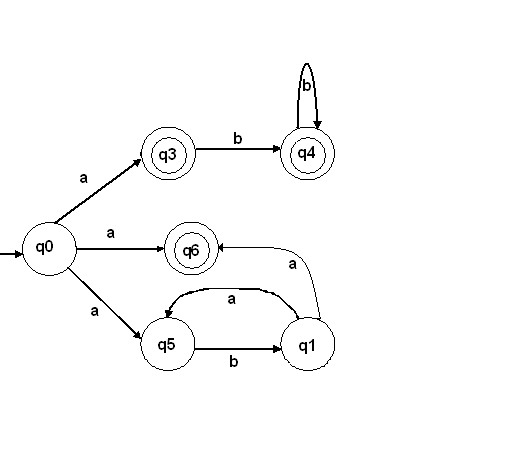
\includegraphics[width=0.6\linewidth]{auto.jpg}}
\caption[Пример диаграммы перехода конечного автомата]{Пример диаграммы перехода конечного автомата}
\label{pic:auto}
\end{figure}

\textit{Диаграмма переходов} (см. рис.~\ref{pic:auto}) для ДКА вида $A = \langle Q, \Sigma, \delta, q_0, F  \rangle$ есть граф, определяемый следующим образом:
\begin{itemize}
 \item [a)] всякому состоянию из $Q$ соответствует некоторая вершина;
 \item [б)] пусть $\delta(q, a) = p$ для некоторого состояния $q$ из $Q$ и входного символа $a$ из $\Sigma$.
 Тогда диаграмма переходов должна содержать дугу из вершины $q$ в вершину $p$, отмеченную $a$.
 Если существует несколько входных символов, переводящих автомат $A$ из состояния $q$ в состояние $p$, то диаграмма переходов может содержать одну дугу, отмеченную списком этих символов;
 \item [в)] диаграмма содержит стрелку в начальное состояние, отмеченную как \textit{Начало}.
 Эта стрелка не выходит не из какого состояния;
 \item [г)] вершины, соответствующие допускающим состояниям (состояниям из $F$), отмечаются двойным кружком.
 Состояния, не принадлежащие $F$, изображаются простым (одинарным) кружком.
\end{itemize}


\textit{Таблица переходов} представляет собой обычное табличное представление функции, подобной $\delta$, которая двум значениям ставит в соответствие одно значение.
Строки таблицы соответствуют состояниям, а столбцы --- входным символам.
На пересечении строки, соответствующей состоянию $q$, и столбца, соответствующего символу $a$, находится состояние $\delta(q, a)$. 
\cite{Intro-TA}

\begin{Def}
Автомат называется \textit{полностью определенным} или \textit{полным}, если $D_\delta = Q \times \Sigma$.
Иными словами, для любого начального состояния и любой входной последовательности (в пределах алфавита $\Sigma$) однозначно определена выходная последовательность.
\end{Def}

\begin{Def}
Автомат называется \textit{частично определенным} или \textit{частичным}, если функция $\delta$ определена не для всех пар $(q, a) \in Q \times \Sigma$. 
\end{Def}

В табличном задании таких автоматов на месте неопределенных состояний и выходных сигналов ставится прочерк. 
На графе автомата неопределенному состоянию можно поставить в соответствие дополнительную вершину.

Неопределенное состояние автомата называется граничным. 
Дальнейшее поведение автомата, попавшего в граничное состояние, не определяется. 
Выходная последовательность, содержащая неопределенные сигналы, называется частичной.
Заметим, что модель частичного автомата является более абстрактной, чем модель полного автомата: она задает целое множество дискретных устройств. \cite{TA-Syntes}

Под \textit{композицией элементарных автоматов} в общем случае понимается следующее.
Пусть заданы элементарные автоматы $A_1, A_2, \dots, A_k$.
Произведем объединение элементарных автоматов в систему совместно работающих автоматов. 
Введем в рассмотрение некоторое конечное множество узлов, называемых внешними выходными узлами. 
Эти узлы отличаются от узлов рассматриваемых элементарных автоматов, которые носят название внутренних.
Композиция автомата состоит в том, что в полученной системе элементарных автоматов $A_1, A_2, \dots, A_k$ и внешних узлов производится отождествление некоторых узлов (как внешних так и внутренних). 

С точки зрения совместной работы системы автоматов смысл операции отождествления узлов состоит в том, что элементарный сигнал, попадающий на один из узлов, входящих в множество отождествляемых между собой узлов, попадает тем самым на все узлы этого множества. 
После проведенных отождествлений узлов система автоматов превращается в так называемую схему (сеть) автоматов.
Будем считать, что автоматы, входящие в систему автоматов, работают совместно, если в каждый момент автоматного времени на все внешние входные узлы подается набор входных сигналов (структурный входной сигнал схемы) и со всех внешних выходных узлов снимается набор выходных сигналов (структурный выходной сигнал). 
Следует заметить, что при построении схемы автоматов должны выполняться условия корректности. 
\cite{TA-Lupal}

\section{Применения автоматной модели для описания процесса перегрузки реактора}

Исходя из положений, представленных в предидущих разделах, представим реактор как композицию конечных детерминированных автоматов.

Пусть реактор состоит из $k$ структурных элементов, каждый из которых можно представить как конечный детерминированный автомат.
Таким образом $i-$й структурный элемент реактора описывается кортежем $A_i = \langle Q^i, \Sigma^i, \delta^i, q_0^i, F^i  \rangle$. 

Тогда реактор можно представить следующим кортежем $A = \langle Q, \Sigma, \delta, q_0, F  \rangle$, где
\begin{itemize}
 \item [-] $Q = \cup_{i=0}^n Q^i$;
 \item [-] $\Sigma = \cup_{i=0}^n \Sigma^i$;
 \item [-] $\delta = f (q, a)$;
 \item [-] $q_0 = \cup_{i=0}^n q_0^i$;
 \item [-] $F = \cap_{i=0}^n F^i$.
\end{itemize}

Рассмотрим данную модель на примере фиктивного реактора.
Пусть реактор имеет следующую конфигурацию активной зоны (см. рис.~\ref{pic:fict-grid}).
Ячейки А1, Б1, В1, Г1, Д1, Е1 предназначены для организации внутриреакторного хранилища отработавших ТВС, 
ячейки А2, Б2, В2, Г2, Д2, Е2 содержат сборки для организации боковой зоны воспроизводства, ячейки А3, Б3, В3, Г3, Д3, Е3 содержат сборки активной зоны реактора и ячейка А4 содержит механизм автоматического регулирования реактора.
\begin{figure}[ht]
\center{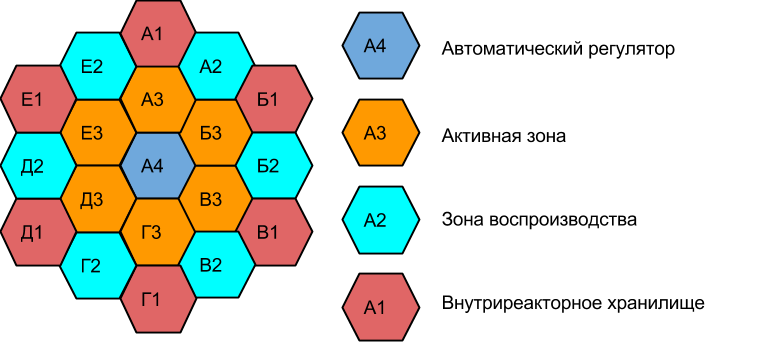
\includegraphics[width=\linewidth]{fict-grid}}
\caption[Конфигурация активной зоны фиктивного реактора]{Конфигурация активной зоны фиктивного реактора: A1 -- внутриреакторное хранилище, А2 -- зона воспроизводства, А3 --- активная зона, А4 --- автоматический регулятор}
\label{pic:fict-grid}
\end{figure}

Фиктивный реактор имеет механизм перегрузки, аналогичный описанному в \ref{BN-PPM}.
Большая поворотная пробка имеет 6 положений, которые соответствуют букве в названии ячейки, малая поворотная пробка - 4 положения, которые соответствуют цифре в названии ячейки.

Перед началом планово-профилактического ремонта поворотные пробки находятся в положении А1, активная зона и зоны воспроизводства  полностью заполнены, внутриреакторное хранилище пусто, частично или полностью заполнено.
Некоторые ТВС активной зоны и зоны воспроизводства, а также все ТВС из внутриреакторного хранилищ помечены как требующие перезагрузки. 
После планово-профилактического ремонта поворотные пробки находятся в положении А1, активная зона и зоны воспроизводства  полностью заполнены, внутриреакторное хранилище пусто, частично или полностью заполнено.
Все ТВС активной зоны и зоны воспроизводства, а также все ТВС из внутриреакторного хранилищ помечены как не требующие перезагрузки. 

Разделим реактор на следующие структурные компоненты: тепловыделяющие сборки с обогащенным ураном, тепловыделяющие сборки с обедненным ураном, гнезда внутриреакторного хранилища, гнезда зоны воспроизводства, гнезда активной зоны, большая поворотная пробка, малая поворотная пробка, перегрузочный механизм.
Рассмотрим отдельные структурные компоненты реактора как автоматы.

\textbf{Тепловыделяющие сборки с обогащенным ураном}:
\begin{itemize}
 \item [-] $Q = \{\text{В активную зону}, \text{Во внутриреакторное хранилище}, \text{Во внешнее хранилище}, \\ \text{Обслуживание завершено}\}$;
 \item [-] $\Sigma = \{\text{Обслужить}\}$;
 \item [-] $\delta = f (q, a)$, где $f$ соответствует таблице~\ref{tab:EFuel};
 \item [-] $q_0 \in \{\text{В активную зону}, \text{Во внутриреакторное хранилище}, \text{Во внешнее хранилище}, \\ \text{Обслуживание завершено}\}$;
 \item [-] $F = \{\text{Обслуживание завершено}\}$.
\end{itemize}

\begin{table} [htbp]
  \centering
  \parbox{15cm}{\caption{Таблица переходов автомата <<Тепловыделяющая сборка с обогащенным ураном>>}\label{tab:EFuel}}
  \begin{center}
  \begin{tabular}{| c | c |}
  \hline
  $q_i \diagdown \sigma_j$& Обслужить \\
  \hline
  В активную зону & Обслуживание завершено\\
  \hline
  Во внутриреакторное хранилище & Обслуживание завершено\\
  \hline
  Во внешнее хранилище& Обслуживание завершено\\
  \hline
  Обслуживание завершено & ---\\
  \hline
  \end{tabular}
  \end{center}
\end{table}

\textbf{Тепловыделяющие сборки с обедненным ураном}:
\begin{itemize}
 \item [-] $Q = \{\text{В зону воспроизводства}, \text{Во внешнее хранилище}, \text{Обслуживание завершено}\}$;
 \item [-] $\Sigma = \{\text{Обслужить}\}$;
 \item [-] $\delta = f (q, a)$, где $f$ соответствует таблице~\ref{tab:DFuel};
 \item [-] $q_0 \in \{\text{В зону воспроизводства}, \text{Во внешнее хранилище}, \text{Обслуживание завершено}\}$;
 \item [-] $F = \{\text{Обслуживание завершено}\}$.
\end{itemize}

\begin{table} [htbp]
  \centering
  \parbox{15cm}{\caption{Таблица переходов автомата <<Тепловыделяющая сборка с обедненным ураном>>}\label{tab:DFuel}}
  \begin{center}
  \begin{tabular}{| c | c |}
  \hline
  $q_i \diagdown \sigma_j$& Обслужить \\
  \hline
  В зону воспроизводства & Обслуживание завершено\\
  \hline
  Во внешнее хранилище& Обслуживание завершено\\
  \hline
  Обслуживание завершено & ---\\
  \hline
  \end{tabular}
  \end{center}
\end{table}

\textbf{Гнезда внутриреакторного хранилища}:
\begin{itemize}
 \item [-] $Q =  A_{ef} \cup \varnothing$, где $A_{ef}$ -- множество автоматов <<Тепловыделяющая сборка с обогащенным ураном>>;
 \item [-] $\Sigma =  A_{ef} \cup \varnothing$, где $A_{ef}$ -- множество автоматов <<Тепловыделяющая сборка с обогащенным ураном>>;
 \item [-] $\delta = f (q, a)$, где $f$ соответствует таблице~\ref{tab:PlaceIn};
 \item [-] $q_0 \in Q$;
 \item [-] $F \in Q$.
\end{itemize}

\begin{table} [htbp]
  \centering
  \parbox{15cm}{\caption{Таблица переходов автомата <<Гнездо внутриреакторного хранилища>>}\label{tab:PlaceIn}}
  \begin{center}
  \begin{tabular}{| c | c | c |}
  \hline
  $q_i \diagdown \sigma_j$& $a_{ef}$ & $\varnothing$ \\
  \hline
  $a_{ef}$&  --- & $\varnothing$\\
  \hline
  $\varnothing$ & $a_{ef}$ & ---\\
  \hline
  \end{tabular}
  \end{center}
\end{table}

\textbf{Гнезда зоны воспроизводства}:
\begin{itemize}
 \item [-] $Q =  A_{uf} \cup \varnothing$, где $A_{uf}$ -- множество автоматов <<Тепловыделяющая сборка с обедненным ураном>>;
 \item [-] $\Sigma =  A_{uf} \cup \varnothing$, где $A_{uf}$ -- множество автоматов <<Тепловыделяющая сборка с обедненным ураном>>;
 \item [-] $\delta = f (q, a)$, где $f$ соответствует таблице~\ref{tab:PlaceRes};
 \item [-] $q_0 \in A_{uf} $;
 \item [-] $F \in A_{uf} $.
\end{itemize}

\begin{table} [htbp]
  \centering
  \parbox{15cm}{\caption{Таблица переходов автомата <<Гнездо зоны воспроизводства>>}\label{tab:PlaceRes}}
  \begin{center}
  \begin{tabular}{| c | c | c |}
  \hline
  $q_i \diagdown \sigma_j$& $a_{uf}$ & $\varnothing$ \\
  \hline
  $a_{uf}$&  --- & $\varnothing$\\
  \hline
  $\varnothing$ & $a_{uf}$ & ---\\
  \hline
  \end{tabular}
  \end{center}
\end{table}

\textbf{Гнезда активной зоны}:
\begin{itemize}
 \item [-] $Q =  A_{ef} \cup \varnothing$, где $A_{ef}$ -- множество автоматов <<Тепловыделяющая сборка с обогащенным ураном>>;
 \item [-] $\Sigma =  A_{ef} \cup \varnothing$, где $A_{ef}$ -- множество автоматов <<Тепловыделяющая сборка с обогащенным ураном>>;
 \item [-] $\delta = f (q, a)$, где $f$ соответствует таблице~\ref{tab:PlaceAct};
 \item [-] $q_0 \in A_{ef} $;
 \item [-] $F \in A_{ef} $.
\end{itemize}

\begin{table} [htbp]
  \centering
  \parbox{15cm}{\caption{Таблица переходов автомата <<Гнездо активной зоны>>}\label{tab:PlaceAct}}
  \begin{center}
  \begin{tabular}{| c | c | c |}
  \hline
  $q_i \diagdown \sigma_j$& $a_{ef}$ & $\varnothing$ \\
  \hline
  $a_{ef}$&  --- & $\varnothing$\\
  \hline
  $\varnothing$ & $a_{ef}$ & ---\\
  \hline
  \end{tabular}
  \end{center}
\end{table}


\textbf{Большая поворотная пробка}:
\begin{itemize}
 \item [-] $Q = \{\text{А}, \text{Б}, \text{В}, \text{Г}, \text{Д}, \text{Е}\}$;
 \item [-] $\Sigma = \{\text{влево}, \text{вправо}\}$;
 \item [-] $\delta = f (q, a)$, где $f$ соответствует таблице~\ref{tab:BP};
 \item [-] $q_0 = \text{А}$;
 \item [-] $F = \text{А}$.
\end{itemize}

\begin{table} [htbp]
  \centering
  \parbox{15cm}{\caption{Таблица переходов автомата <<Большая поворотная пробка>>}\label{tab:BP}}
  \begin{center}
  \begin{tabular}{| c | c | c |}
  \hline
  $q_i \diagdown \sigma_j$& влево & вправо \\
  \hline
  А & Е & Б\\
  \hline
  Б & А & В\\
  \hline
  В & Б & Г\\
  \hline
  Г & В & Д\\
  \hline
  Д & Г & Е\\
  \hline
  Е & Д & А\\
  \hline
  \end{tabular}
  \end{center}
\end{table}



\textbf{Малая поворотная пробка}:
\begin{itemize}
 \item [-] $Q = \{1, 2, 3, 4\}$;
 \item [-] $\Sigma = \{\langle \text{влево}, q_{bp}\rangle, \langle \text{вправо}, q_{bp}\rangle\}$, где $q_{bp}$ -- текущее состояние автомата <<Большая поворотная пробка>>;
 \item [-] $\delta = f (q, a)$, где $f$ соответствует таблице~\ref{tab:SP};
 \item [-] $q_0 = 1$;
 \item [-] $F = 1$.
\end{itemize}

\begin{table} [htbp]
  \centering
  \parbox{15cm}{\caption{Таблица переходов автомата <<Малая поворотная пробка>>}\label{tab:SP}}
  \begin{center}
  \begin{tabular}{| c | c | c | c | c |}
  \hline
  $q_i \diagdown \sigma_j$ & $\langle \text{влево}, \text{А} \rangle$ & $\langle \text{вправо}, \text{А}\rangle$ & $\langle \text{влево}, \overline{\text{А}}\rangle$ & $\langle \text{вправо}, \overline{\text{А}}\rangle$\\
  \hline
  1 &4&2&3&2\\
  \hline
  2 &1&3&1&3\\
  \hline
  3 &2&4&2&1\\
  \hline
  4 &3&1&-&-\\
  \hline
  \end{tabular}
  \end{center}
\end{table}

\textbf{Перегрузочный механизм}:
Рассмотрим перегрузочный механизм как совокупность следующих автоматов: большая поворотная пробка, малая поворотная пробка, определитель типа гнезда, селектор гнезда, перегрузочный механизм.

\textit{Определитель типа гнезда}:
\begin{itemize}
 \item [-] $Q = \{\text{Внутриреакторное хранилище}, \text{Зона воспроизводства}, \text{Активная зона},\\
 \text{Автоматический регулятор}\}$;
 \item [-] $\Sigma = \{1, 2, 3, 4\}$;
 \item [-] $\delta = f (q, a)$, где $f$ соответствует таблице~\ref{tab:Determinator};
 \item [-] $q_0 = \text{Внутриреакторное хранилище}$;
 \item [-] $F = \text{Внутриреакторное хранилище}$.
\end{itemize}
\begin{table} [htbp]
  \centering
  \parbox{15cm}{\caption[Таблица переходов автомата <<Определитель типа гнезда>>]{Таблица переходов автомата <<Определитель типа гнезда>>: ВХ -- Внутриреакторное хранилище; ЗВ -- Зона воспроизводства; АЗ -- Активная зона; АР -- Автоматический регулятор.}\label{tab:Determinator}}
  \begin{center}
  \begin{tabular}{| c | c | c | c | c |}
  \hline
  $q_i \diagdown \sigma_j$ & 1 & 2 & 3& 4\\
  \hline
  ВХ& ВХ& ЗВ& АЗ& АР\\
  \hline
  ЗВ& ВХ& ЗВ& АЗ& АР\\
  \hline
  АЗ& ВХ& ЗВ& АЗ& АР\\
  \hline
  АР& ВХ& ЗВ& АЗ& АР\\
  \hline
  \end{tabular}
  \end{center}
\end{table}

\textit{Селектор гнезда}:
\begin{itemize}
 \item [-] $Q = Q_{\text{гнезда}}$;
 \item [-] $\Sigma = \langle Q_{\text{A1}},\dots, Q_{\text{Е3}}, Q_{bp}, Q_{lp}\rangle$;
 \item [-] $\delta = f (q, a)$, где $f$ соответствует таблице~\ref{tab:Selector};
 \item [-] $q_0 = Q_{\text{A1}}$;
 \item [-] $F = Q_{\text{A1}}$.
\end{itemize}

\begin{table} [htbp]
  \centering
  \parbox{15cm}{\caption{Таблица переходов автомата <<Селектор гнезда>>.}\label{tab:Selector}}
  \begin{center}
  \begin{tabular}{| c | c | c | c |}
  \hline
  $q_i \diagdown \sigma_j$ & $\langle q_{\text{A1}},\dots, q_{\text{Е3}}, \text{A}, 1\rangle$ & $\cdots$ & 
  $\langle q_{\text{A1}},\dots, q_{\text{Е3}}, \text{Е}, 3\rangle$\\
  \hline
  $\forall q \in Q$& $q_{\text{A1}}$ & $\cdots$ & $q_{\text{Е3}}$\\
  \hline
  \end{tabular}
  \end{center}
\end{table}

\textit{Перегрузочный механизм}:
\begin{itemize}
 \item [-] $Q = A_{\text{ТВС}} \cup \varnothing$;
 \item [-] $\Sigma = \langle Q_{\text{Селектора}},\dots, Q_{\text{Определителя}}, \{\text{извлечь}, \text{установить}, \text{во внешнее хранилище},\\ \text{из внешнего хранилища}\}\rangle$;
 \item [-] $\delta = f (q, a)$, где $f$ соответствует таблице~\ref{tab:Elevator};
 \item [-] $q_0 = \varnothing$;
 \item [-] $F = \varnothing$.
\end{itemize}

\begin{table} [htbp]
  \centering
  \parbox{15cm}{\caption[Таблица переходов автомата <<Перегрузочный механизм>>]{Таблица переходов автомата <<Перегрузочный механизм>>: ВХ -- Внутриреакторное хранилище; ВнешХ -- Внешнее хранилище; ЗВ -- Зона воспроизводства; АЗ -- Активная зона; АР -- Автоматический регулятор.}\label{tab:Elevator}}
  \begin{center}
  \begin{tabular}{| c | c | c | c | c | c | }
  \hline
  $\sigma_j \diagdown q_i$ & $\varnothing$ & В АЗ & Во ВХ & Во внешХ & В ЗВ\\
  \hline
  $\langle \varnothing, \text{АЗ}, \text{извлечь}\rangle$&---&---&---&---&---\\
  \hline
  $\langle \varnothing, \text{АЗ}, \text{установить}\rangle$&---&$\varnothing$&---&---&---\\
  \hline
  $\langle \varnothing, \text{АЗ}, \text{во внешнее хранилище}\rangle$&---&---&---&---&---\\
  \hline
  $\langle \varnothing, \text{АЗ}, \text{из внешнего хранилища}\rangle$&$A_{\text{ТВС}}$&---&---&---&---\\
  \hline
  $\cdots$&$\cdots$&$\cdots$&$\cdots$&$\cdots$&$\cdots$\\
  \hline
  $\langle \text{В ЗВ}, \text{ВХ}, \text{из внешнего хранилища}\rangle$&---&---&---&---&---\\
  \hline
  \end{tabular}
  \end{center}
\end{table}

Рассмотрев отдельные автоматы, моделирующие поведение структурных элементов реактора, рассмотрим композицию этих автоматов (ТА-модель).
Согласно описанию фиктивного реактора, приведенного выше (см. рис.~\ref{pic:fict-grid}), ТА-модель реактора состоит из $6-12$ ТА-моделей тепловыделяющих сборок с обогащенным ураном, $6$ ТА-моделей тепловыделяющих сборок с обедненным ураном, $6$ ТА-моделей гнезд активной зоны, $6$ ТА-моделей гнезд зоны воспроизводства, $6$ ТА-моделей гнезд внутриреакторного хранилища, ТА-модели большой поворотной пробки, ТА-модели малой поворотной пробки, ТА-модели селектора гнезд, ТА-модели определителя типа гнезда и ТА-модели перегрузочного механизма.    

Выходы ТА-моделей ТВС с обогащенным ураном являются входными символами для ТА-моделей гнезд активной зоны и ТА-моделей гнезд внутриреакторного хранилища. 
Выходы ТА-моделей ТВС с обедненным ураном являются входными символами для ТА-модели гнезд зоны воспроизводства. 
Выходы ТА-моделей гнезд реактора являются входными символами ТА-модели селектора гнезд. 
Выход ТА-модели большой поворотной пробки является входным символом для ТА-моделей малой поворотной пробки, селектора гнезд и определителя типа гнезд.
Выход ТА-модели малой поворотной пробки является входным символом для ТА-модели селектора гнезд и определителя типа гнезд.
Выходы ТА-моделей селектора гнезд и определителя типа гнезд являются входными символами для ТА-модели перегрузочного механизма.
Композиционная схема ТА-модели фиктивного реактора представлена на рисунке~\ref{pic:fict-composition}.

\begin{figure}[ht]
\center{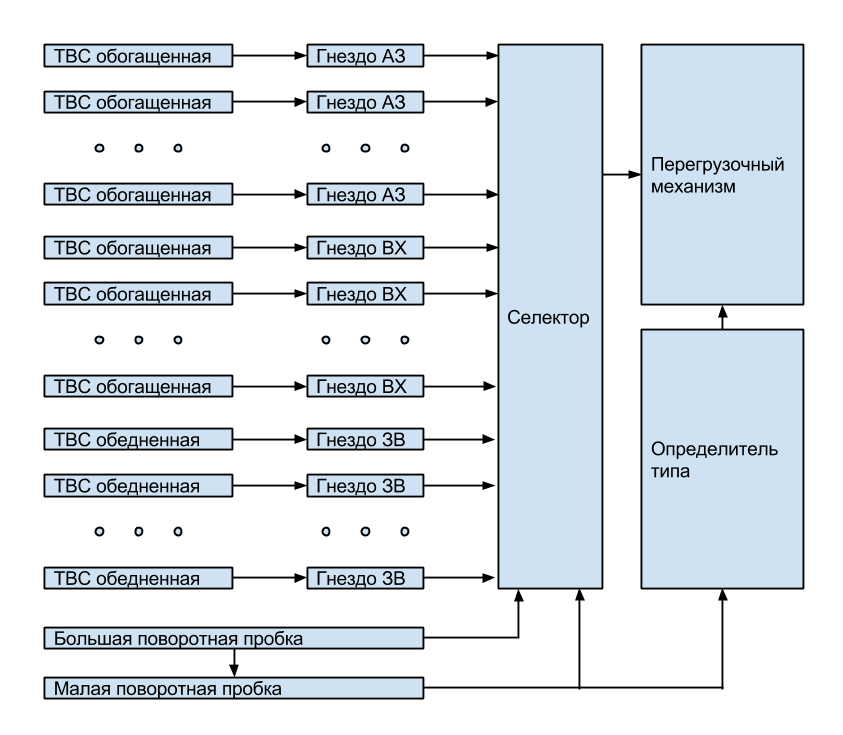
\includegraphics[width=\linewidth]{fict-composition}}
\caption[Композиционная схема автоматов модели фиктивного реактора]{Композиционная схема автоматов модели фиктивного реактора: ТВС -- тепловыделющая сборка, ВХ -- Внутриреакторное хранилище; ЗВ -- Зона воспроизводства; АЗ -- Активная зона.}
\label{pic:fict-composition}
\end{figure}

Исходя из описанного выше представим модель фиктивного реактора в общем виде следующим образом:
\begin{itemize}
 \item [-] $Q = \langle Q_{\text{ТВС 1}}, \dots, Q_{\text{ТВС 18}}, Q_{\text{A1}},\dots, Q_{\text{Е3}}, Q_{bp}, Q_{lp}, Q_{\text{перегрузочного механизма}} \rangle$;
 \item [-] $\Sigma = \{\text{извлечь}, \text{установить}, \text{во внешнее хранилище}, \text{из внешнего хранилища},\\ \text{БПП влево}, \text{БПП вправо}, \text{МПП влево}, \text{МПП вправо}\}$;
 \item [-] $\delta = \delta_{\text{ТВС 1}} \cdot \dots \cdot  \delta_{\text{ТВС 18}} \cdot  \delta_{\text{A1}} \cdot \dots \cdot \delta_{\text{Е3}} \cdot  \delta_{bp} \cdot  \delta_{lp} \cdot \delta_{\text{перегрузочного механизма}}$;
 \item [-] $q_0 = \langle q_{\text{ТВС 1}}, \dots, q_{\text{ТВС 18}}, q_{\text{A1}},\dots, q_{\text{Е3}}, q_{bp}, q_{lp}, q_{\text{перегрузочного механизма}} \rangle$;
 \item [-] $F = \langle F_{\text{ТВС 1}}, \dots, F_{\text{ТВС 18}}, F_{\text{A1}},\dots, F_{\text{Е3}}, F_{bp}, F_{lp}, F_{\text{перегрузочного механизма}} \rangle$.
\end{itemize}

\section{Выводы по главе}

В данной главе сформулирована постановка задачи оптимизации технологического процесса.
Предложен общий подход к решению задачи оптимизации технологического процесса.
Определены следующие входные данные: описание конструкции реактора, данные для физического моделирования и функция оптимизации.
В качестве выходных данных определн оптимальный порядок технологического процесса.

Рассмотрены основные положения теории автоматов.
Введено понятие автоматной модели (ТА-модели).
Рассмотрен подход к построению композиции ТА-моделей.

Показан пример построения ТА-модели фиктивного реактора.